\documentclass{beamer}
\usepackage{./fl_slides}
\usepackage{./mathoperatorsAuD}

\usepackage{csquotes}
\usepackage{amsmath,amssymb}
\usepackage{enumerate}
\usepackage[inline]{enumitem} 		%customize label
\newcommand{\labelitemi}{\raisebox{1pt}{\scalebox{.9}{$\blacktriangleright$}}}
\newcommand{\labelitemii}{$\vartriangleright$}
\newcommand{\labelitemiii}{--}

\usepackage{multicol}

\usepackage{booktabs}
\usepackage{tabularx}
\usepackage{tabu}
\newcommand*\head{\rowfont{\bfseries}}
\newcommand*{\tw}{\rowfont{\ttfamily}}

\renewcommand{\tabularxcolumn}[1]{>{\hspace{0pt}}m{#1}}

\newcommand{\person}[1]{\textsc{#1}}

\title{Formal Languages}
\subtitle{with Respect to the \person{Chomsky}-\person{Schützenberger}-Hierarchy}
\author{Eric Kunze}
\city{TU Dresden}
%\institute{Lehrstuhl für Grundlagen der Programmierung}
\titlegraphic{
\includegraphics[width=2cm]{./TUD-white.pdf}}

\AtBeginSection[]
{
	\begin{frame}
		\frametitle{Contents}
		\bfseries
		\tableofcontents[currentsection]
	\end{frame}
}
\setbeamertemplate{section in toc}{%
	\leavevmode\leftskip=1.75ex%
	\llap{%
		\usebeamerfont*{section number projected}%
		\usebeamercolor[bg]{section number projected}%
		\vrule width2.25ex height1.85ex depth.4ex%
		\hskip-2.25ex%
		\hbox to2.25ex{\hfil\color{fg}\inserttocsectionnumber\hfil}}%
	\kern1.25ex\inserttocsection\par}

\DeclareMathOperator{\lat}{lat}
\DeclareMathOperator{\bin}{bin}
\DeclareMathOperator{\countL}{count}

\renewcommand{\emph}[1]{\textbf{#1}}

\begin{document}	
	
	\maketitle
	
	\setbeamertemplate{section in toc}[square]
	
	\begin{frame} \frametitle{Contents}
		\bfseries
		\tableofcontents
	\end{frame}
	
	
	\section{Introduction}
	
	\begin{frame} \frametitle{Syntax vs. Semantic}
		\textbf{\enquote{Colorless green ideas sleep furiously.}}
		
		\pause
		
		\begin{figure}
			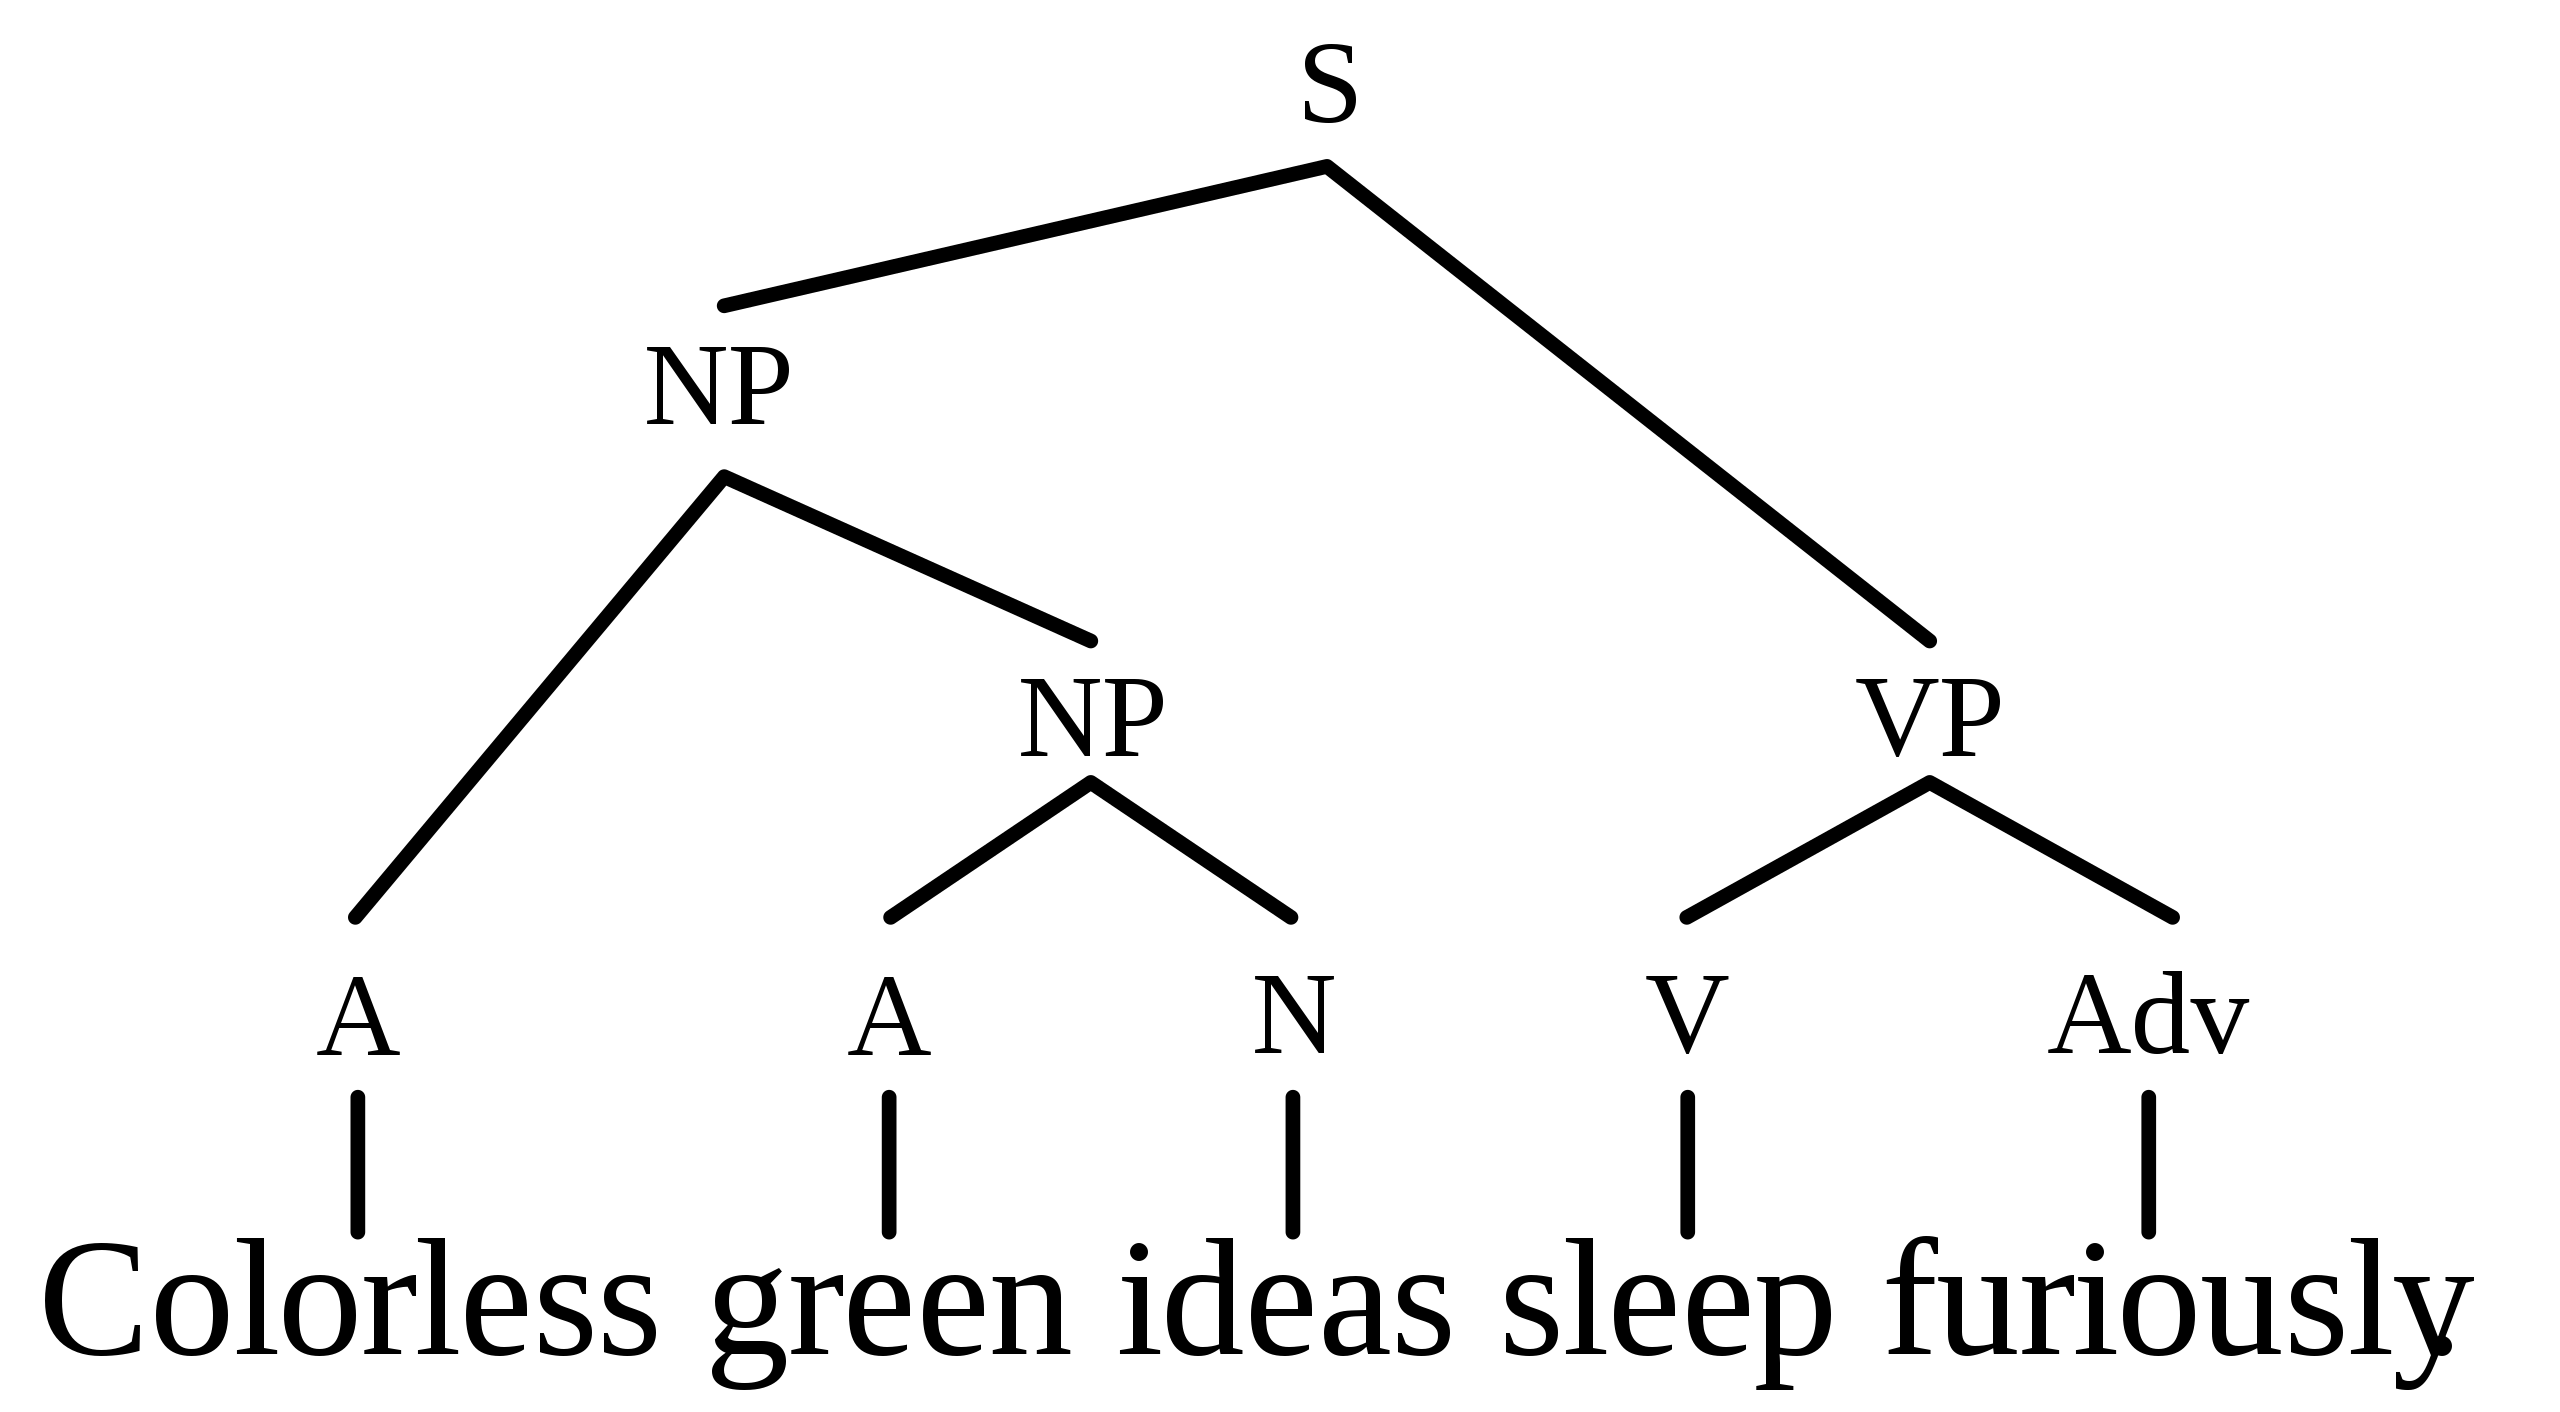
\includegraphics[height=10em]{fl_ex1.png}
			\caption{Tree representation of the sentence structure \cite{chomskySyntax}}
		\end{figure}
	
		\pause
	
		\person{\textbf{Noam Chomsky}} (* December 7, 1928) \\
		\enquote{father of modern linguistics}
	\end{frame}


	\begin{frame} \frametitle{Formal Language}
		\Large
		\alert<3>{\onslide<4>{$\vert$} i \ s \ \alert<2>{o} \ m \ o \ r \ p \ h \ i \ s \ m \onslide*<4>{$\vert = 11$}} \onslide<6>{\ $\in L_{\text{eng}}$} \onslide*<5>{$\in$} \onslide*<6>{$\subset$} \onslide<5-6>{$\Sigma_{\lat}^\ast$} \\
		
		\normalsize
		\begin{itemize}
			\item<2-> \textbf{alphabet} $\Sigma$ --- set of symbols
			\item<3-> \textbf{word} $w$ over $\Sigma$ --- finite sequence of symbols
			\item<4-> \textbf{length} $\abs{w}$ --- number of symbols of $w$
			\item<5-> \textbf{Kleene-Star} $\Sigma^\ast$ --- set of all words over $\Sigma$
			\item<6-> \textbf{(formal) language} $L \subseteq \Sigma^\ast$ --- set of (selected) words over $\Sigma$
		\end{itemize}
	\end{frame}

	\begin{frame} \frametitle{Simple Examples}
		\begin{itemize}
			\item<+-> $\N_0 = \menge{\epsilon, 1, 11, 111, \dots}$ over $\Sigma = \menge{1}$
			\item<+-> $\countL_2 = \menge{a^n b^n : n \in \N}$ over $\Sigma = \menge{a,b}$
			\item<+-> $\countL_3 = \menge{a^n b^n c^n : n \in \N}$ over $\Sigma = \menge{a, b, c}$
			\item<+-> programming language $C$
			\begin{itemize}
				\item alphabet: valid keywords and symbols
				\item words: valid programs
			\end{itemize}
		\end{itemize}
	\end{frame}


	\section{Formal Grammar}
	\begin{frame} \frametitle{Formal Grammar}
		\textbf{How to form strings over a given alphabet $\Sigma$?}
		\pause
		\begin{itemize}
			\item accept words --- automata theory
			\item generate words --- theory of grammar
		\end{itemize}
		
		\pause
		
		\begin{definition}[Grammar]
			A (formal) grammar $G$ is a 4-tuple $(N, \Sigma, P, S)$ where
			\begin{itemize}
				\item $N$ and $\Sigma$ are finite, disjoint sets of symbols (alphabets) 
				\item elements of $N$ are called non-terminal symbols, \\
				elements of $\Sigma$ are called terminal symbols
				\item $P$ is a set of productions $(N \cup \Sigma)^\ast N (N \cup \Sigma)^\ast \to (N \cup \Sigma)^\ast$
				\item $S \in N$ is the start symbol
			\end{itemize}
		\end{definition}
	\end{frame}

% 	\begin{frame} \frametitle{Formal Grammar}
%		Let $G = (N, \Sigma, P, S)$ be a formal grammar.
%		
%		\pause
%		
%		\textbf{Interpretation}:
%		\begin{itemize}
%			\item $N$ ... symbols which can be replaced
%			\item $\Sigma$ ... symbols occuring in words
%			\item $P$ ... rules \textit{how} we can replace
%			\item $S$ ... (non-terminal) symbol we have to start with
% 		\end{itemize}
% 	
% 		\pause
% 	
% 		\textbf{Convention}: We denote
% 		\begin{itemize}
% 			\item elements of $N$ with capitals ($S,A,B,C, \dots$)
% 			\item elements of $\Sigma$ with small letters ($a,b,c,d \dots$)
% 		\end{itemize}
%	\end{frame}

	\begin{frame} \frametitle{Example}
		\begin{example}
			$G = (N,\Sigma, P, S)$ where $N = \menge{S}$, $\Sigma = \menge{a,b}$ and $P = \menge{S \to aSb, S \to ab}$.
		\end{example}
	
		\pause
		
%		\begin{definition}
%			The language of a grammar $G = (N,\Sigma, P, S)$, denoted by $L(G)$, is the set of all words which can be derived in a finite number of steps applying rules from $P$ starting with $S$. \\
%			$\blacktriangleright$ \textit{Write $\vdash^k_{(i)}$ for the $k$-fold application of rule $(i)$.}
%		\end{definition}
%		\begin{example}
			\textbf{Produced words over $\Sigma$:} \\
			$\menge{ab,aabb,aaabbb, \dots} = \countL_2$
%		\end{example}

%		\pause
%		\begin{example}
%			$G = (N, \Sigma, P, S)$ where $N = \menge{S,A,B}$, $\Sigma = \menge{a,b,c}$ and $P$ consists of the following rules: \\[-4em]		
%			\begin{multicols}{3}
%				\begin{itemize}
%					\item \upshape{(1)} $\quad S \to abc$ 
%					\item \upshape{(2)} $\quad S \to aSBc$
%					\item \upshape{(3)} $\quad cB \to Bc$
%					\item \upshape{(4)} $\quad bB \to bb$
%				\end{itemize}
%			\end{multicols}
%		\end{example}
%		\pause
%		\textbf{Produced words over $\Sigma$:} \\
%		$\menge{abc,aabbcc,aaabbbccc, \dots} = \countL_3$
	\end{frame}

	

	\section{Chomsky-Schützenberger Hierarchy}
	
%	\begin{frame} \frametitle{Chomsky-Hierarchy}
%		\begin{itemize}
%			\item \textbf{aim:} classify languages $L(G)$
%			\item \textbf{method:} 
%			\begin{itemize}
%				\item classify grammar $G = (N,\Sigma,P,S)$ 
%				\item classify set of productions $P$
%			\end{itemize}
%		\end{itemize}
%	\end{frame}

	\begin{frame} \frametitle{Chomsky-Hierarchy \cite{baader}}
		Let $G = (N,\Sigma,P,S)$ be a formal grammar. 
		Then $G$ is a \textbf{type-0-grammar}. \pause $G$ is called a
		\begin{itemize}
			\item \textbf{type-1-grammar} (\textit{context-sensitive}) if every production has the form
			\begin{itemize}
				\item $u_1 A u_2 \to u_1 w u_2$ where $A \in N$, $u_1, u_2, w \in (N \cup \Sigma)^\ast$ and $\abs{w} \ge 1$ or
				\item $S \to \epsilon$
			\end{itemize} 
			Is $(S \to \epsilon) \in P$, so $S$ never appears on a production's right side.
		\end{itemize}
	
		\pause
	
		\begin{example}[$L(G) = \countL_3$]
			Let $N = \menge{S,A,B}$, $\Sigma = \menge{a,b,c}$ and $P$ consist of the following rules: \\[-1em]	
			\begin{multicols}{3}
				\begin{itemize}
					\item \upshape{(1)} $\quad S \to abc$ 
					\item \upshape{(2)} $\quad S \to aSBc$
					\item \upshape{(3)} $\quad cB \to Bc$
					\item \upshape{(4)} $\quad bB \to bb$
				\end{itemize}
			\end{multicols}
		\end{example}
%		\textbf{Example:}  $L(G) = \countL_3$ \\
%		Let $N = \menge{S,A,B}$, $\Sigma = \menge{a,b,c}$ and $P$ consists of the following rules: \\[-1em]	
%		\begin{multicols}{3}
%			\begin{itemize}
%				\item \upshape{(1)} $\quad S \to abc$ 
%				\item \upshape{(2)} $\quad S \to aSBc$
%				\item \upshape{(3)} $\quad cB \to Bc$
%				\item \upshape{(4)} $\quad bB \to bb$
%			\end{itemize}
%		\end{multicols}
	\end{frame}

	\begin{frame} \frametitle{Chomsky-Hierarchy \cite{baader}}
		Let $G = (N,\Sigma,P,S)$ be a formal grammar. $G$ is called a
		\begin{itemize}
			\item \textbf{type-2-grammar} (\textit{context-free}) if every production has the form $A \to w$ where $A \in N$ and $w \in (N \cup \Sigma)^\ast$
		\end{itemize}
	
		\pause
		
		\begin{example}[$L(G) = \countL_2$]
			Let $N = \menge{S}$, $\Sigma = \menge{a,b}$ and
			\begin{equation*}
			P = \menge{S \to aSb, S \to ab}
			\end{equation*} 
		\end{example}
%		\textbf{Example:} $L(G) = \countL_2$. \\
%		Let $N = \menge{S}$, $\Sigma = \menge{a,b}$ and
%		\begin{equation*}
%			P = \big\{ \underbrace{S \to aSb}_{(1)}, \underbrace{S \to ab}_{(2)} \big\}
%		\end{equation*} 
	\end{frame}

	\begin{frame} \frametitle{Chomsky-Hierarchy \cite{baader}}
		Let $G = (N,\Sigma,P,S)$ be a formal grammar. $G$ is called a
		\begin{itemize}
			\item \textbf{type-3-grammar} (\textit{regular}) if every production has the form
			$A \to uB$ oder $A \to u$ where $A,B \in N$ and $u \in \Sigma^\ast$
		\end{itemize}
	
		\begin{example}[$L(G) = \N_0$]
			Let $N = \menge{S}$, $\Sigma = \menge{1}$, 
			\begin{equation*}
			P = \menge{S \to \epsilon, \ S \to 1S}
			\end{equation*}
		\end{example}
%		\texon*}
	\end{frame}
	
	\section{Applications}
	
	\begin{frame} \frametitle{Applications}
		\begin{itemize}
			\item<+-> \textbf{syntax of programming languages} \\
			e.g. \texttt{if}-condition in $C$
				\begin{equation*}
					\begin{aligned}
					ifStat &\to \texttt{if} \ ( \ BoolExp \ ) \ Stat \\
					ifStat &\to \texttt{if} \ ( \ BoolExp \ ) \ Stat \ \texttt{else} \ Stat
					\end{aligned}
				\end{equation*}
			\item<+-> \textbf{mathematical logic}
			\begin{itemize}
				\item (propositional) logic as formal language $L_{\log}$ over alphabet $\Sigma = \menge{p_1, p_2, \dots} \cup \menge{\lnot, \land, \lor, (,)}$
				\item words: valid formulae --- e.g. $(\lnot (p_1 \lor p_2) \land p_3) \in L_{\log}$
			\end{itemize}
			\item<+-> \textbf{Computability Theory}
			\begin{itemize}
				\item Which problem is computable with which machine?
%				\item \textbf{\person{Church}-\person{Turing} thesis:} \textit{Any real-world computation can be translated into an equivalent computation involving a Turing machine.}
			\end{itemize}
		\end{itemize}
	\end{frame}

%%%%%%%%%%%%%%%%%%%%%%%%%%%%%%%%%%%%%%%%%%%%%%%%%%%%%%%%%%%%%%%%%%%%%%%%%%%%%%%%%%%

	\begin{frame}[shrink=30] \frametitle{References}
%		\renewcommand*{\bibfont}{\scriptsize}
		\nocite{*}	
		\bibliographystyle{abbrv}
		\bibliography{FL_bib_p}
	\end{frame}

%%%%%%%%%%%%%%%%%%%%%%%%%%%%%%%%%%%%%%%%%%%%%%%%%%%%%%%%%%%%%%%%%%%%%%%%%%%%%%%%%%%
	
	\appendix
	\begin{frame}
	\end{frame}

	\begin{frame} \frametitle{Formal Language}
		\begin{itemize}
			\item<+-> \emph{alphabet} $\Sigma$ --- set of symbols
			\begin{itemize}
				\item latin alphabet $\Sigma_{\lat} = \menge{a, b, \dots, z}$
				\item binary alphabet $\Sigma_{\bin} = \menge{0,1}$
			\end{itemize}
			\item<+-> \emph{word} $w$ over $\Sigma$ --- finite sequence of symbols 
			%		($w = \sigma_1 \sigma_2 \dots \sigma_n$ where $\sigma_1, \sigma_2, \dots, \sigma_n \in \Sigma$)
			\begin{itemize}
				\item $english$ and $sdlfkhui$ are words over $\Sigma_{\lat}$
				\item $01101$ is a word over $\Sigma_{\bin}$, but not over $\Sigma_{\lat}$ 
			\end{itemize}
			\item<+-> \emph{length} $\abs{w}$ --- number of symbols of $w$
			\begin{itemize}
				\item word with length zero: $\epsilon$
				\item $\abs{english} = 7$
			\end{itemize}
			\item<+-> \emph{Kleene-Star} $\Sigma^\ast$ --- set of all words over $\Sigma$
			\item<+-> \emph{(formal) language} $L \subseteq \Sigma^\ast$ --- set of (selected) words over $\Sigma$
		\end{itemize}
	\end{frame}

	\begin{frame} \frametitle{Example --- $\countL_2$}
		\begin{theorem}
			Let $G = (N,\Sigma, P, S)$ where $N = \menge{S}$, $\Sigma = \menge{a,b}$ and
			\begin{equation*}
			P = \big\{ \underbrace{S \to aSb}_{(1)}, \underbrace{S \to ab}_{(2)} \big\}
			\end{equation*} 
			Then $L(G) = \menge{a^n b^n : n \in \N} = \countL_2$.
		\end{theorem}
		\textbf{Proof.} We just prove that $\countL_2 \subseteq L(G)$, i.e. $a^n b^n \in L(G)$ for all $n \in \N$.
		\begin{itemize}
			\item consideration:
			\begin{equation*}
				\begin{array}{lrllllcl}
				\triangleright \quad & S &\vdash_{(1)} & aSb &\vdash_{(2)} & aabb &=& a^2 b^2 \\
				\triangleright \quad & S &\vdash_{(1)}^2 & a^2 S b^2 &\vdash_{(2)} & a^2 ab b^2 &=& a^3 b^3 \quad \dots
				\end{array}
			\end{equation*}
			\item in general:
			\begin{equation*}
				S \vdash_{(1)}^{n-1} a^{n-1} S b^{n-1} \vdash_{(2)} a^{n-1} a b b^{n-1} = a^n b^n
			\end{equation*}
		\end{itemize}
		%		\begin{itemize}
		%			\item base: $n=0$ --- Starting with $S$ and applying $S \to \epsilon$ we get $a^0 b^0 = \epsilon$.
		%			\item step: assuming that $a^n b^n \in L(G)$
		%			\begin{itemize}
		%				\item proof that $a^{n+1} b^{n+1} \in L(G)$
		%				\item starting with $a^n b^n = a^n \epsilon b^n$ , use $S \to \epsilon$ reverse $\follows a^n S b^n$
		%				\item applying $S \to aSb$ we reach $a^n aSb b^n = a^{n+1} S b^{n+1}$ 
		%				\item with $S \to \epsilon$ we get $a^{n+1} b^{n+1} \in L(G)$
		%			\end{itemize}
		%		\end{itemize}
	\end{frame}
	
	\begin{frame} \frametitle{Example --- $\countL_3$}
		Is there a grammer $G$ with $L(G) = \countL_3 = \menge{a^n b^n c^n : n \in \N}$?
		
		\begin{theorem}
			Let $G = (N, \Sigma, P, S)$ be a formal grammar with $N = \menge{S,A,B}$, $\Sigma = \menge{a,b,c}$ and $P$ consists of the following rules: 		
			\begin{multicols}{3}
				\begin{itemize}
					\item \upshape{(1)} $\quad S \to abc$ 
					\item \upshape{(2)} $\quad S \to aSBc$
					\item \upshape{(3)} $\quad cB \to Bc$
					\item \upshape{(4)} $\quad bB \to bb$
				\end{itemize}
			\end{multicols}
			Then $L(G) = \countL_3$.
		\end{theorem}
		\textbf{Example:} $a^3 b^3 c^3 \in L(G)$?
		\begin{alignat*}{2}
		S \quad &\vdash^2_{(2)} aaSBcBc \quad &\vdash_{(1)} aaabcBcBc \\
		&\vdash_{(3)}^2 aaabBcBcc \quad &\vdash_{(3)}^1 aaabBBccc \\
		&\vdash_{(4)}^2 aaabbbccc
		\end{alignat*}
	\end{frame}

	\begin{frame} \frametitle{Mathematical Logic}
		\begin{itemize}
			\item (propositional) Logic as formal language $L_{\log}$
			\item alphabet: $\Sigma = \menge{p_1, p_2, \dots} \cup \menge{\lnot, \land, \lor, (,)}$
			\item words: 
			\begin{itemize}
				\item $p_1, p_2, \dots \in L_{\log}$
				\item $\lnot f \in L_{\log}$ if $f \in L_{\log}$
				\item $(f_1 \land f_2) \in L_{\log}$ if $f_1, f_2 \in L_{\log}$
				\item $(f_1 \lor f_2) \in L_{\log}$ if $f_1, f_2 \in L_{\log}$
			\end{itemize}
			\item examples:
			\begin{itemize}
				\item $(p_1 \land p_2) \in L_{\log}$
				\item $((\lnot (p_1 \lor p_2) \land p_3) \lor \lnot p_1) \in L_{\log}$
			\end{itemize}
		\end{itemize}
	\end{frame}
	
	\begin{frame} \frametitle{Computability Theory}
		\begin{description}
			\item[Question:]  Which problem is computable with which machine?
			\item[]   
			\item[\fbox{\person{Church}-\person{Turing} thesis}] ~ \\[1em]
			\begin{itshape}
				Any real-world computation can be translated into an equivalent computation involving a Turing machine.
			\end{itshape}
			\item[] 
			\item[Halting Problem:] Decide whether a given (arbitrary) program will finish running or continue to run forever
		\end{description}
	\end{frame}
\end{document}